\documentclass[12pt,a4paper]{article}
\usepackage[utf8]{inputenc}
\usepackage[T1]{fontenc}
\usepackage[polish]{babel}
\usepackage{graphicx}
\usepackage{booktabs}
\usepackage{amsmath}
\usepackage{geometry}
\usepackage{hyperref}
\usepackage{float}
\usepackage{caption}
\usepackage{xcolor}
\usepackage{array}
\usepackage{multirow}
\usepackage{enumitem}

\geometry{margin=2.5cm}

\hypersetup{colorlinks=true,linkcolor=blue!60!black,urlcolor=blue!60!black}

\title{
    \vspace{-1cm}
    \Large\textbf{Anonimizacja danych}\\[0.4em]
    \large k-anonimowość, l-różnorodność, t-bliskość\\
    \large oraz odporność na Atak Skośności \\[0.4em]
    \normalsize Zbiory danych: Adult (UCI) \textperiodcentered{} Medical Cost \textperiodcentered{} German Credit (UCI)
}
\author{Piotr Zapała, Jan Poręba, Maksymilian Neumann}
\date{\today}

\begin{document}

\maketitle
\tableofcontents
\newpage

% =============================================================================
\section{Wprowadzenie}
% =============================================================================

Celem niniejszego sprawozdania jest analiza porównawcza trzech technik
anonimizacji danych tabelarycznych:

\begin{itemize}
    \item \textbf{k-anonimowość} --- każdy rekord jest nieodróżnialny od
          co najmniej $k{-}1$ innych rekordów ze względu na quasi-identyfikatory.
    \item \textbf{l-różnorodność} --- w każdej klasie równoważności atrybut
          wrażliwy przyjmuje co najmniej $l$ dobrze reprezentowanych wartości
          (entropia $H(EC_i) \geq \log l$).
    \item \textbf{t-bliskość} --- rozkład atrybutu wrażliwego w każdej klasie
          jest bliski rozkładowi globalnemu (dystans $\leq t$).
\end{itemize}

Analizę przeprowadzono na trzech zbiorach danych, a wyniki oceniono pod kątem
skuteczności \textbf{Ataku Skośności} .

\subsection{Zbiory danych}

\begin{table}[H]
\centering
\caption{Charakterystyka zbiorów danych}
\begin{tabular}{lclll}
\toprule
\textbf{Dataset} & \textbf{Rekordy} & \textbf{Quasi-identyfikatory} & \textbf{Atr. wrażliwy} & \textbf{Typ} \\
\midrule
Adult (UCI)   & 47\,592 & education\_grp, sex, race, age & income           & 4 warianty \\
Medical Cost  & 1\,337  & sex, region, age, bmi          & charges\_cat     & 4 kwartyle \\
German Credit & 1\,000  & personal\_status, housing,     & checking\_status & 4 kategorie \\
              &         & foreign\_worker, age           &                  & \\
\bottomrule
\end{tabular}
\end{table}

\subsection{Parametry analizy}

Kolumny numeryczne (wiek, BMI) generalizowano metodą kwantylową
(\texttt{pd.qcut}), która równomiernie rozkłada rekordy między kubełki.
Optymalną liczbę kubełków wyznaczano adaptacyjnie.
Próg ataku skośności ustalono na $\tau = 0{,}10$.

% =============================================================================
\section{k-anonimowość}
% =============================================================================

\subsection{Definicja}

Zbiór danych spełnia \textbf{k-anonimowość}, jeśli każda klasa równoważności
$EC_i$ (zbiór rekordów o identycznych wartościach quasi-identyfikatorów)
zawiera co najmniej $k$ rekordów:
\[
    \forall\, i \colon |EC_i| \geq k
\]
Realizacja przez \emph{supresję}: klasy z $|EC_i| < k$ są usuwane w całości.

\subsection{Wyniki adaptacyjnego wyszukiwania}

\begin{table}[H]
\centering
\caption{Optymalne parametry k-anonimowości (l=2, bez t-bliskości)}
\begin{tabular}{lcccc}
\toprule
\textbf{Dataset} & \textbf{k opt.} & \textbf{age\_bins} & \textbf{bmi\_bins} & \textbf{Zachowane [\%]} \\
\midrule
Adult         & 5  & 2 & ---  & 99{,}9\% \\
Medical Cost  & 20 & 2 & 2    & 100{,}0\% \\
German Credit & 2  & 2 & ---  & 97{,}5\% \\
\bottomrule
\end{tabular}
\end{table}

\subsection{Wnioski}

\begin{itemize}
    \item \textbf{Adult}: zbiór duży (47\,592 rek.),
          generalizacja do 2 kubełków wiekowych i 2 klas edukacji
          tworzy naturalnie duże klasy równoważności.
          Przy $k=5$ supresja wynosi zaledwie $0{,}1\%$ --- praktycznie bezstratna.

    \item \textbf{Medical Cost}: mały zbiór (1\,337 rek.), ale tylko 32 klasy.
          Nawet przy $k=20$ każda klasa ma $\geq 25$ rekordów --- brak supresji.

    \item \textbf{German Credit}: najmniejszy zbiór (1\,000 rek.),
          3 kategoryczne QI dają wiele małych klas.
          Przy $k=2$ utrata 2{,}5\% --- dobry wynik, lecz $k=2$
          oznacza słabą ochronę (zaledwie 2 rekordy w klasie).

    \item \textbf{Kluczowa obserwacja}: sama k-anonimowość nie chroni
          przed wnioskowaniem o atrybucie wrażliwym --- klasa z $k=5$
          rekordami może mieć 4 z tą samą wartością atrybutu wrażliwego.
\end{itemize}

% =============================================================================
\section{l-różnorodność}
% =============================================================================

\subsection{Definicja}

Klasa równoważności $EC_i$ spełnia \textbf{l-różnorodność} (entropijną),
jeśli entropia Shannona rozkładu atrybutu wrażliwego jest wystarczająca:
\[
    H(EC_i) = -\sum_{s \in S} P(s|EC_i)\,\log P(s|EC_i) \;\geq\; \log l
\]

\subsection{Wyniki}

\begin{table}[H]
\centering
\caption{Wpływ l-różnorodności na zachowanie rekordów (optymalne k)}
\begin{tabular}{lcccc}
\toprule
\textbf{Dataset} & \textbf{k} & \textbf{l} & \textbf{Zachowane po k} & \textbf{Zachowane po k+l} \\
\midrule
Adult         & 5  & 2 & 100{,}0\% & 99{,}9\% \\
Medical Cost  & 10 & 2 & 100{,}0\% & 100{,}0\% \\
German Credit & 5  & 2 & 97{,}6\%  & 97{,}1\% \\
\bottomrule
\end{tabular}
\end{table}

\subsection{Wnioski}

\begin{itemize}
    \item \textbf{Adult}: income ma 4 warianty (\texttt{<=50K},
          \texttt{<=50K.}, \texttt{>50K}, \texttt{>50K.}) ---
          l-różnorodność spełniona przy supresji tylko $0{,}1\%$.
          Entropia minimalna $0{,}709 > \log 2 = 0{,}693$.

    \item \textbf{Medical Cost}: charges\_cat pochodzi z \texttt{qcut},
          każda kategoria ma globalnie $\approx 25\%$ rekordów.
          Klasy naturalnie spełniają $l=2$ --- brak supresji.

    \item \textbf{German Credit}: checking\_status ma nierównomierny rozkład
          (39\% \texttt{no account}, 6\% \texttt{>=200 DM}).
          Supresja $0{,}5\%$ --- l-różnorodność działa efektywnie.

    \item \textbf{Kluczowa obserwacja}: l-różnorodność \emph{nie chroni}
          przed atakiem skośności gdy globalny rozkład atrybutu jest
          równomierny (Medical Cost) --- entropia może być wysoka,
          a rozkład lokalny nadal silnie odbiega od globalnego.
\end{itemize}

% =============================================================================
\section{t-bliskość}
% =============================================================================

\subsection{Definicja}

Klasa $EC_i$ spełnia \textbf{t-bliskość}, jeśli dystans między rozkładem
atrybutu wrażliwego w klasie a rozkładem globalnym nie przekracza $t$:
\[
    d\bigl(P(S|EC_i),\; P(S)\bigr) \;\leq\; t
\]
Dla atrybutów kategorycznych stosujemy \emph{dystans wariacyjny}
$\frac{1}{2}\sum_s |P_i(s) - P_G(s)|$,
dla numerycznych \emph{Earth Mover's Distance} (EMD).

\subsection{Adaptacyjne wyszukiwanie optymalnego (k, l, t)}

\begin{table}[H]
\centering
\caption{Optymalne parametry z t-bliskością}
\begin{tabular}{lcccccc}
\toprule
\textbf{Dataset} & \textbf{k} & \textbf{l} & \textbf{t} & \textbf{age\_bins} & \textbf{bmi\_bins} & \textbf{Zachowane [\%]} \\
\midrule
Adult         & 5  & 2 & 0{,}30 & 2 & ---  & 89{,}1\% \\
Medical Cost  & 10 & 2 & 0{,}30 & 2 & 2    & 62{,}2\% \\
German Credit & 5  & 2 & 0{,}30 & 2 & ---  & 96{,}2\% \\
\bottomrule
\end{tabular}
\end{table}

\subsection{Wnioski}

\begin{itemize}
    \item We wszystkich trzech datasetach optymalne $t = 0{,}30$,
          zachowując odpowiednio 89\%, 62\% i 96\% rekordów.
    \item \textbf{Medical Cost} traci 38\% rekordów przy $t=0{,}30$ ---
          wynika to z dużej demograficznej różnorodności kosztów leczenia.
    \item \textbf{German Credit} traci tylko 4\% przy $t=0{,}30$ ---
          najlepszy kompromis spośród trzech datasetów.
\end{itemize}

% =============================================================================
\section{Atak skośności }
% =============================================================================

\subsection{Opis ataku}

Atak skośności wykorzystuje fakt, że rozkład atrybutu wrażliwego
w klasie równoważności może istotnie różnić się od rozkładu globalnego.
Atakujący, znając quasi-identyfikatory ofiary, wyznacza jej klasę
i porównuje histogram lokalny z globalnym:
\[
    \text{atak udany} \iff \exists\, s \colon |P_i(s) - P_G(s)| > \tau
\]
Przy $\tau = 0{,}10$ każde odchylenie powyżej 10 pkt. proc.
uznawane jest za wyciek informacji.

\subsection{Wyniki pipeline'u}

\begin{table}[H]
\centering
\caption{Skuteczność ataku skośności po kolejnych etapach anonimizacji}
\begin{tabular}{llcccc}
\toprule
\textbf{Dataset} & \textbf{Etap} & \textbf{Rekordy} & \textbf{Klas} & \textbf{Podatnych} & \textbf{Max odch.} \\
\midrule
\multirow{3}{*}{Adult}
  & k=5               & 100{,}0\% & 40 & 28 (70{,}0\%) & 0{,}306 \\
  & k=5, l=2          & 99{,}9\%  & 39 & 27 (69{,}2\%) & 0{,}306 \\
  & k=5, l=2, t=0{,}3 & 89{,}1\%  & 35 & 19 (54{,}3\%) & 0{,}272 \\
\midrule
\multirow{3}{*}{Medical Cost}
  & k=10               & 100{,}0\% & 32 & 32 (100{,}0\%) & 0{,}364 \\
  & k=10, l=2          & 100{,}0\% & 32 & 32 (100{,}0\%) & 0{,}364 \\
  & k=10, l=2, t=0{,}3 & 62{,}2\%  & 19 & 19 (100{,}0\%) & 0{,}307 \\
\midrule
\multirow{3}{*}{German Credit}
  & k=5               & 97{,}6\%  & 20 & 13 (65{,}0\%) & 0{,}271 \\
  & k=5, l=2          & 97{,}1\%  & 19 & 12 (63{,}2\%) & 0{,}272 \\
  & k=5, l=2, t=0{,}3 & 96{,}2\%  & 18 & 12 (66{,}7\%) & 0{,}199 \\
\bottomrule
\end{tabular}
\end{table}

\subsection{Wykresy analizy podatności}

\begin{figure}[H]
    \centering
    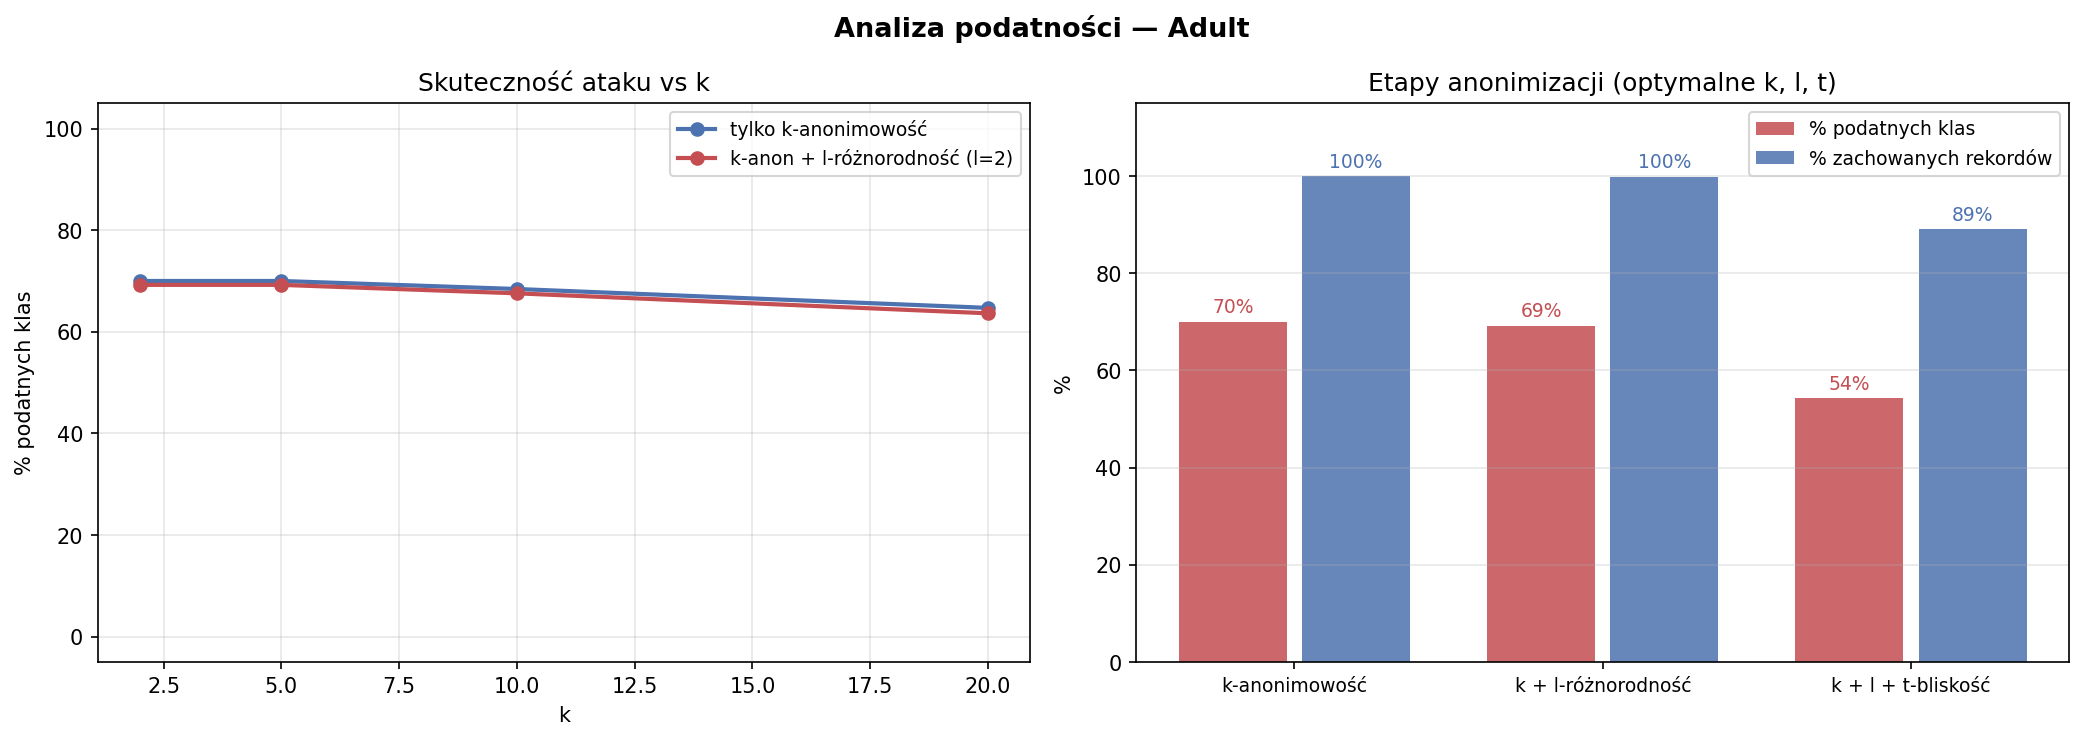
\includegraphics[width=\textwidth]{../plots/full_analysis_adult.png}
    \caption{Adult --- lewy panel: \% podatnych klas vs $k$ dla k-anonimowości
             i k+l-różnorodności. Obie krzywe prawie się pokrywają --- l-różnorodność
             nie poprawia ochrony przed atakiem. Prawy panel: porównanie trzech
             etapów pipeline dla optymalnych $k=5$, $l=2$, $t=0{,}3$.}
\end{figure}

\begin{figure}[H]
    \centering
    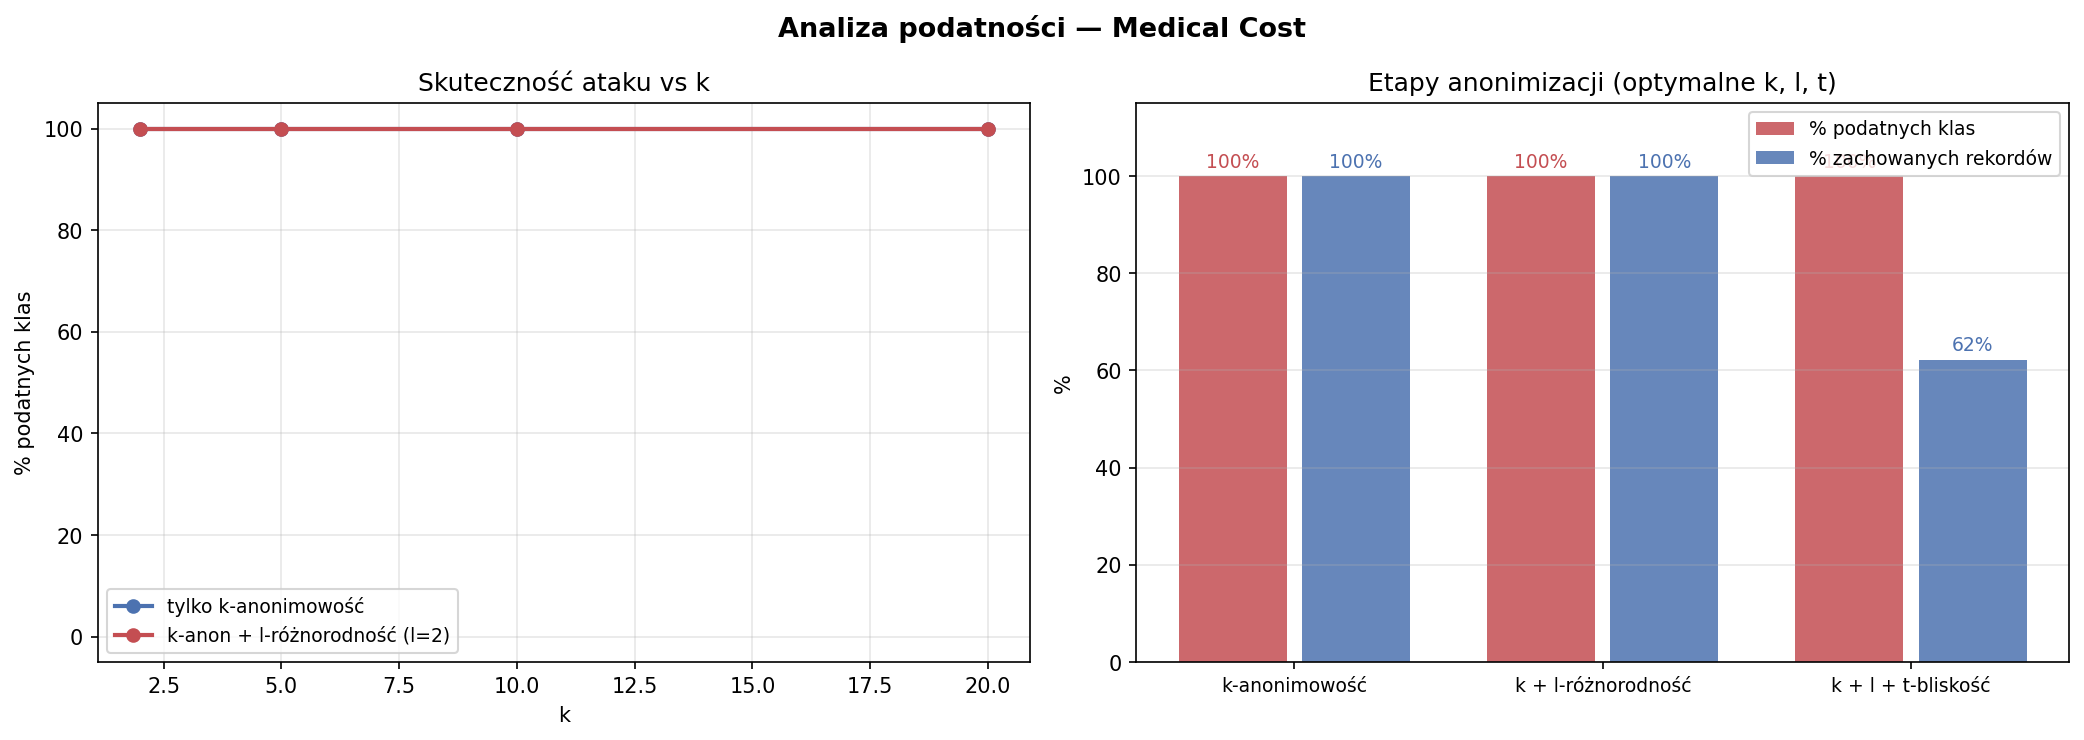
\includegraphics[width=\textwidth]{../plots/full_analysis_medical_cost.png}
    \caption{Medical Cost --- lewy panel: podatność stale 100\% niezależnie od $k$ i $l$.
             Prawy panel: dopiero t-bliskość ($t=0{,}3$) redukuje rekordy do 62\%,
             ale podatność pozostaje 100\%.}
\end{figure}

\begin{figure}[H]
    \centering
    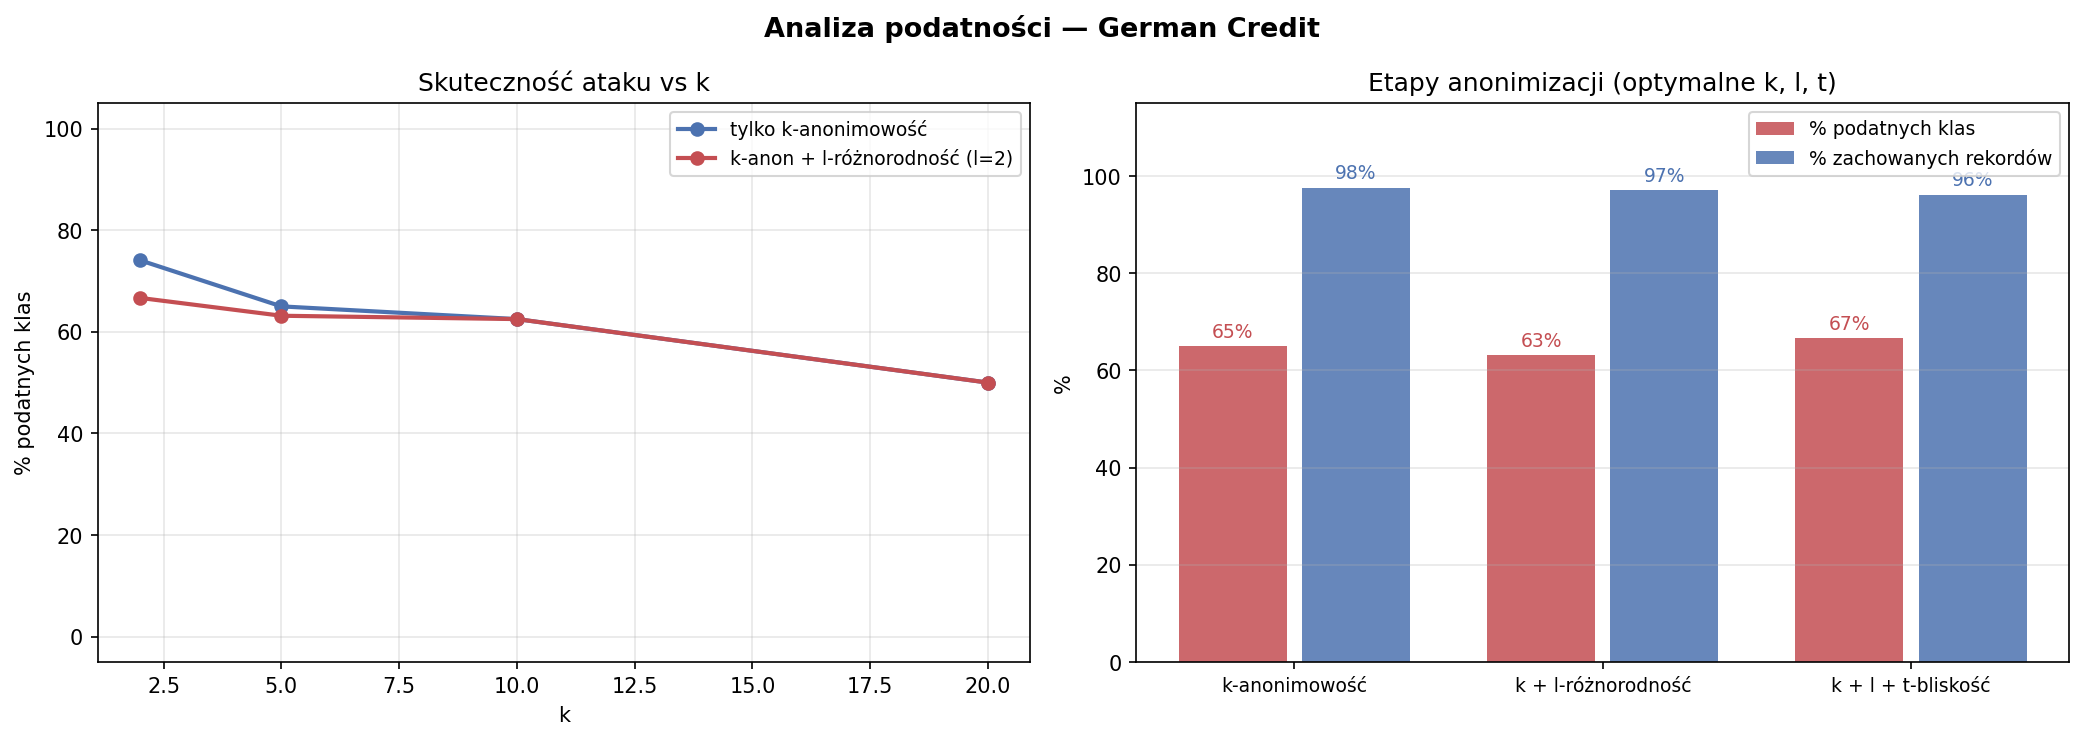
\includegraphics[width=\textwidth]{../plots/full_analysis_german_credit.png}
    \caption{German Credit --- lewy panel: podatność maleje z $k$, l-różnorodność
             daje nieznaczną poprawę. Prawy panel: t-bliskość nie redukuje
             znacząco rekordów (96\%), ale też nie eliminuje ataku.}
\end{figure}

\subsection{Wykresy ataku po każdym etapie --- Adult}

\begin{figure}[H]
    \centering
    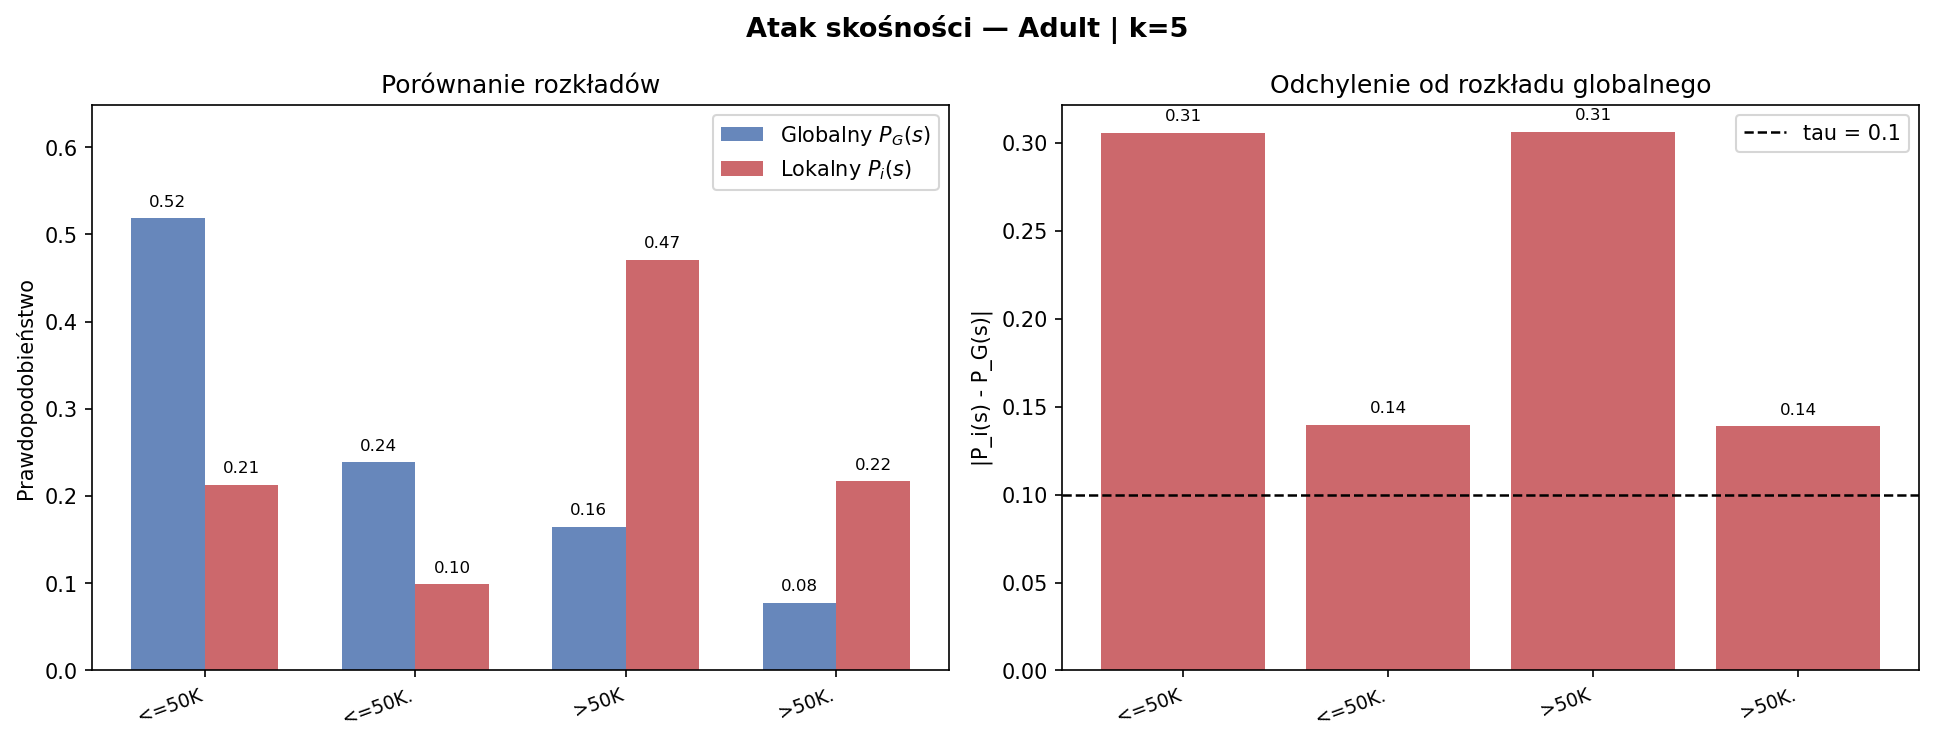
\includegraphics[width=\textwidth]{../plots/attack_adult_k5.png}
    \caption{Adult po k-anonimowości ($k=5$). Najbardziej podatna klasa:
             (Higher educ., Male, White, starszy wiek) ---
             $P_i(\texttt{>50K}) = 0{,}47$ vs $P_G(\texttt{>50K}) = 0{,}16$,
             odchylenie 0{,}31.}
\end{figure}

\begin{figure}[H]
    \centering
    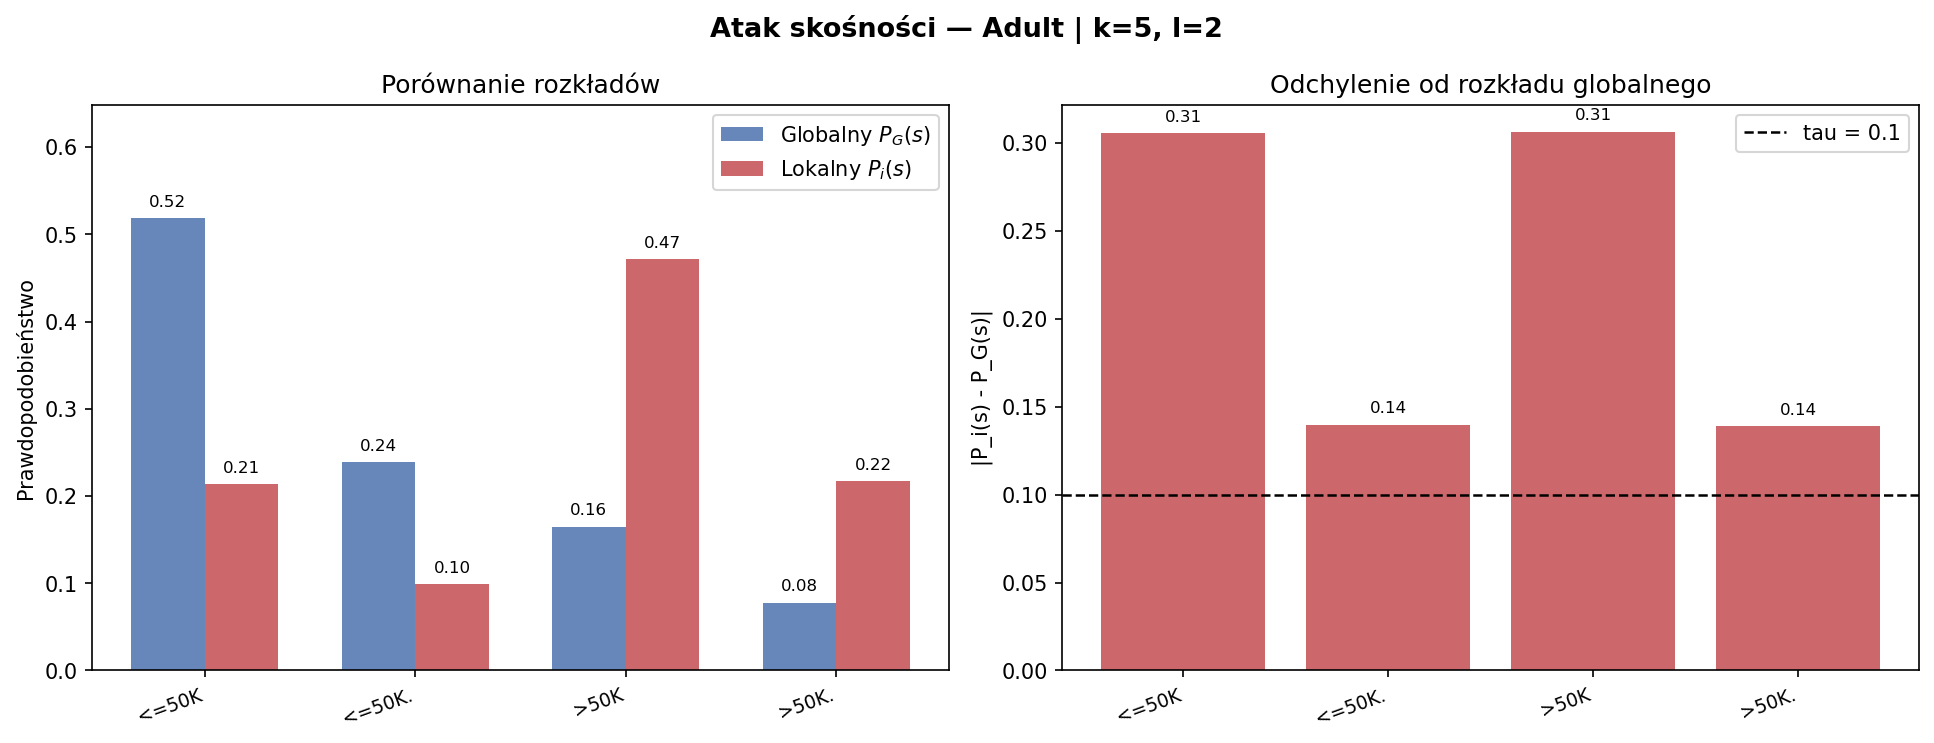
\includegraphics[width=\textwidth]{../plots/attack_adult_k5_l2.png}
    \caption{Adult po l-różnorodności ($l=2$). Liczba podatnych klas spada
             z 28 do 27 --- l-różnorodność prawie nie pomaga.
             Najbardziej podatna klasa pozostaje ta sama.}
\end{figure}

\begin{figure}[H]
    \centering
    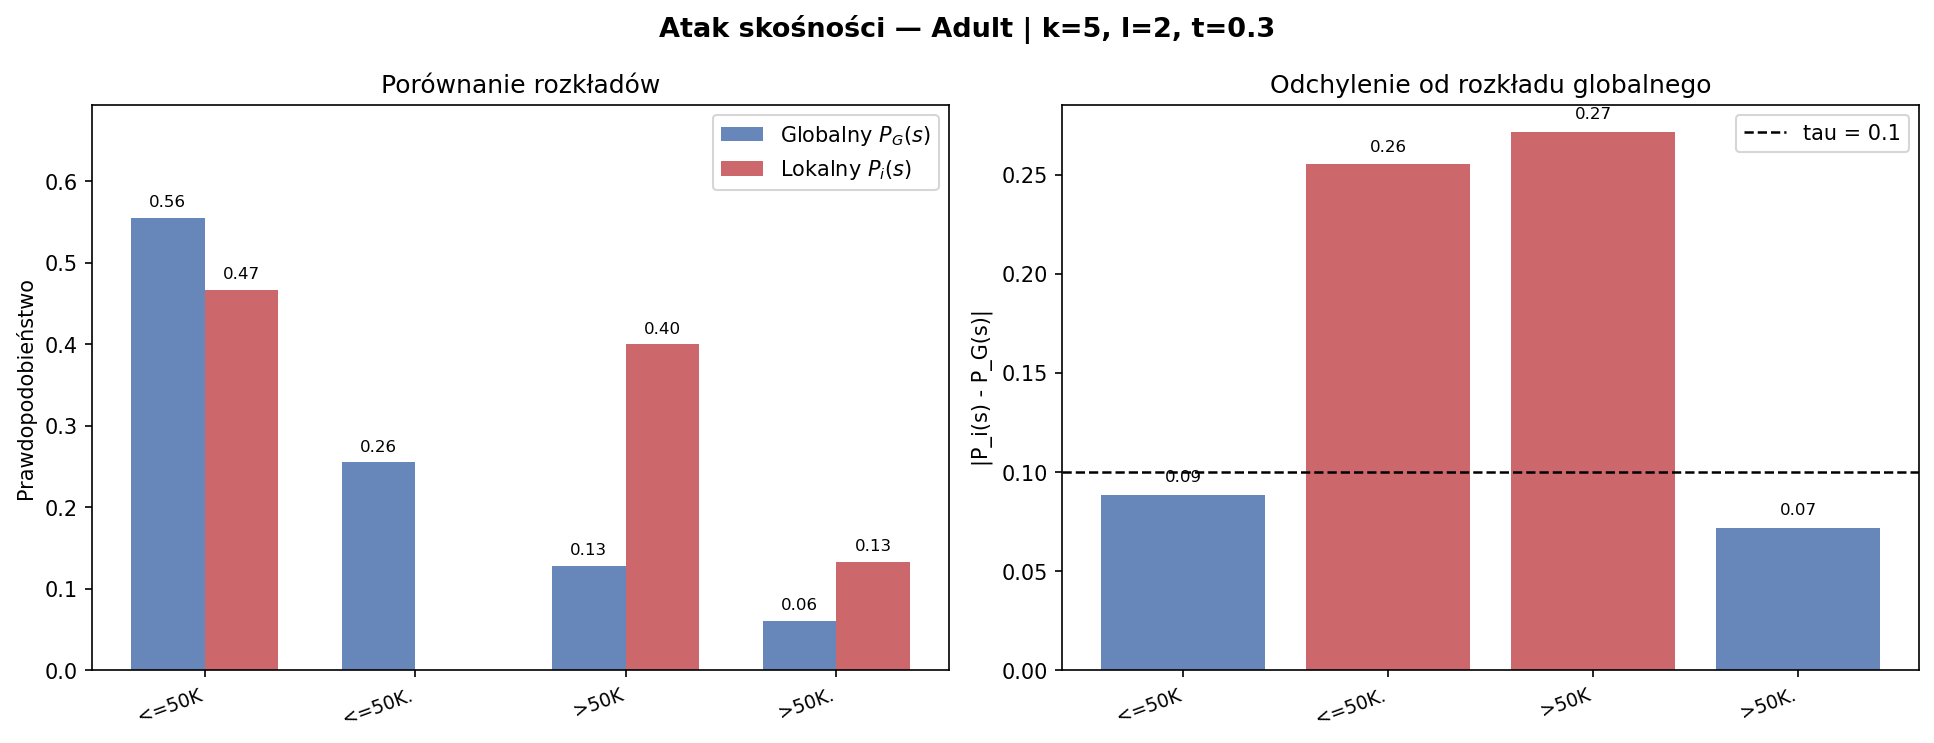
\includegraphics[width=\textwidth]{../plots/attack_adult_k5_l2_t0.3.png}
    \caption{Adult po t-bliskości ($t=0{,}3$). Podatnych klas 19 (54\%) ---
             atak nadal skuteczny. Max odchylenie 0{,}27 $> \tau=0{,}10$.
             Atak dotyczy teraz innej klasy: (Higher, Male, Amer-Indian-Eskimo).}
\end{figure}

\subsection{Wykresy ataku po każdym etapie --- Medical Cost}

\begin{figure}[H]
    \centering
    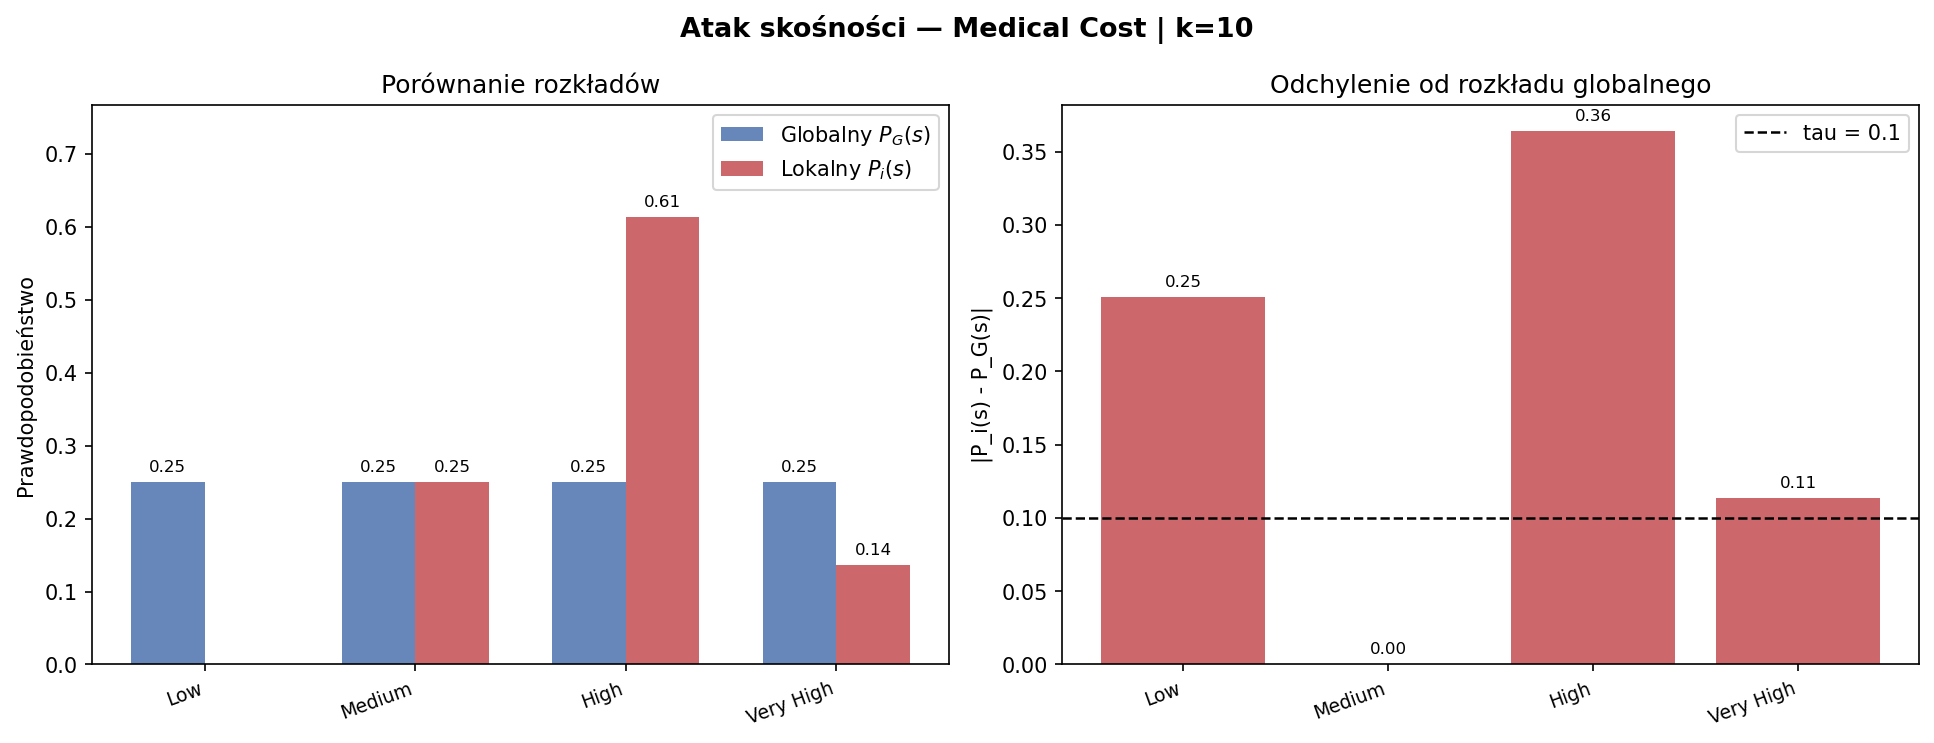
\includegraphics[width=\textwidth]{../plots/attack_medical_cost_k10.png}
    \caption{Medical Cost po k-anonimowości ($k=10$). Wszystkie 32 klasy podatne (100\%).
             Podatna klasa (female, southwest, starszy, wyższe BMI):
             \texttt{High}=0{,}61 vs 0{,}25 globalnie.}
\end{figure}

\begin{figure}[H]
    \centering
    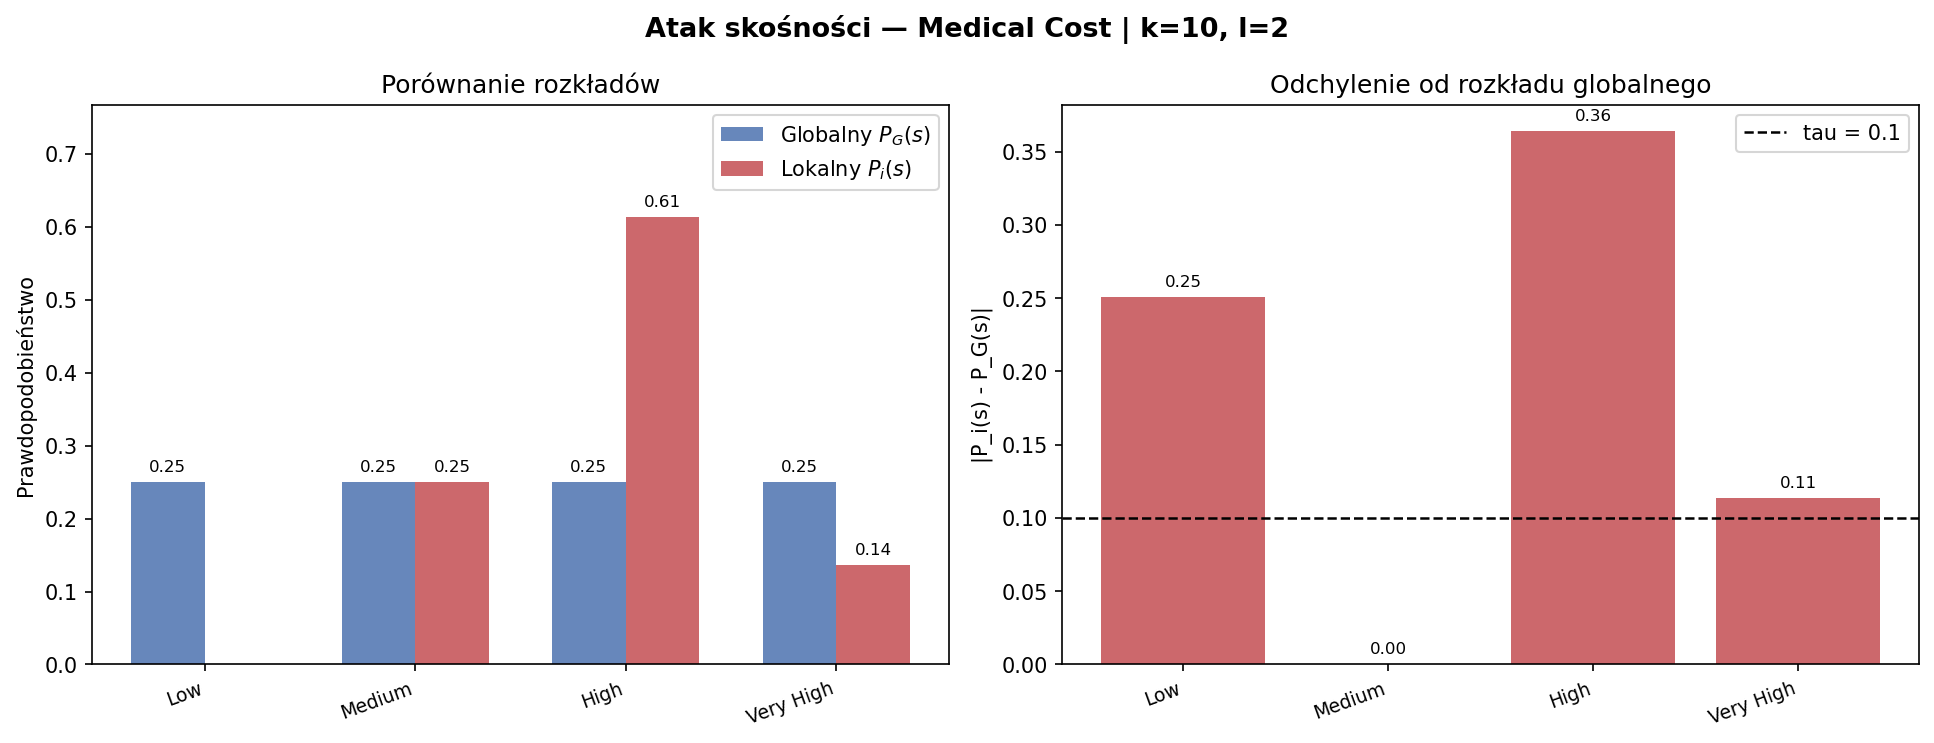
\includegraphics[width=\textwidth]{../plots/attack_medical_cost_k10_l2.png}
    \caption{Medical Cost po l-różnorodności ($l=2$). Identyczny wynik ---
             100\% klas podatnych. charges\_cat jest równomierny globalnie,
             więc entropia w każdej klasie jest wysoka mimo lokalnej dominacji.}
\end{figure}

\begin{figure}[H]
    \centering
    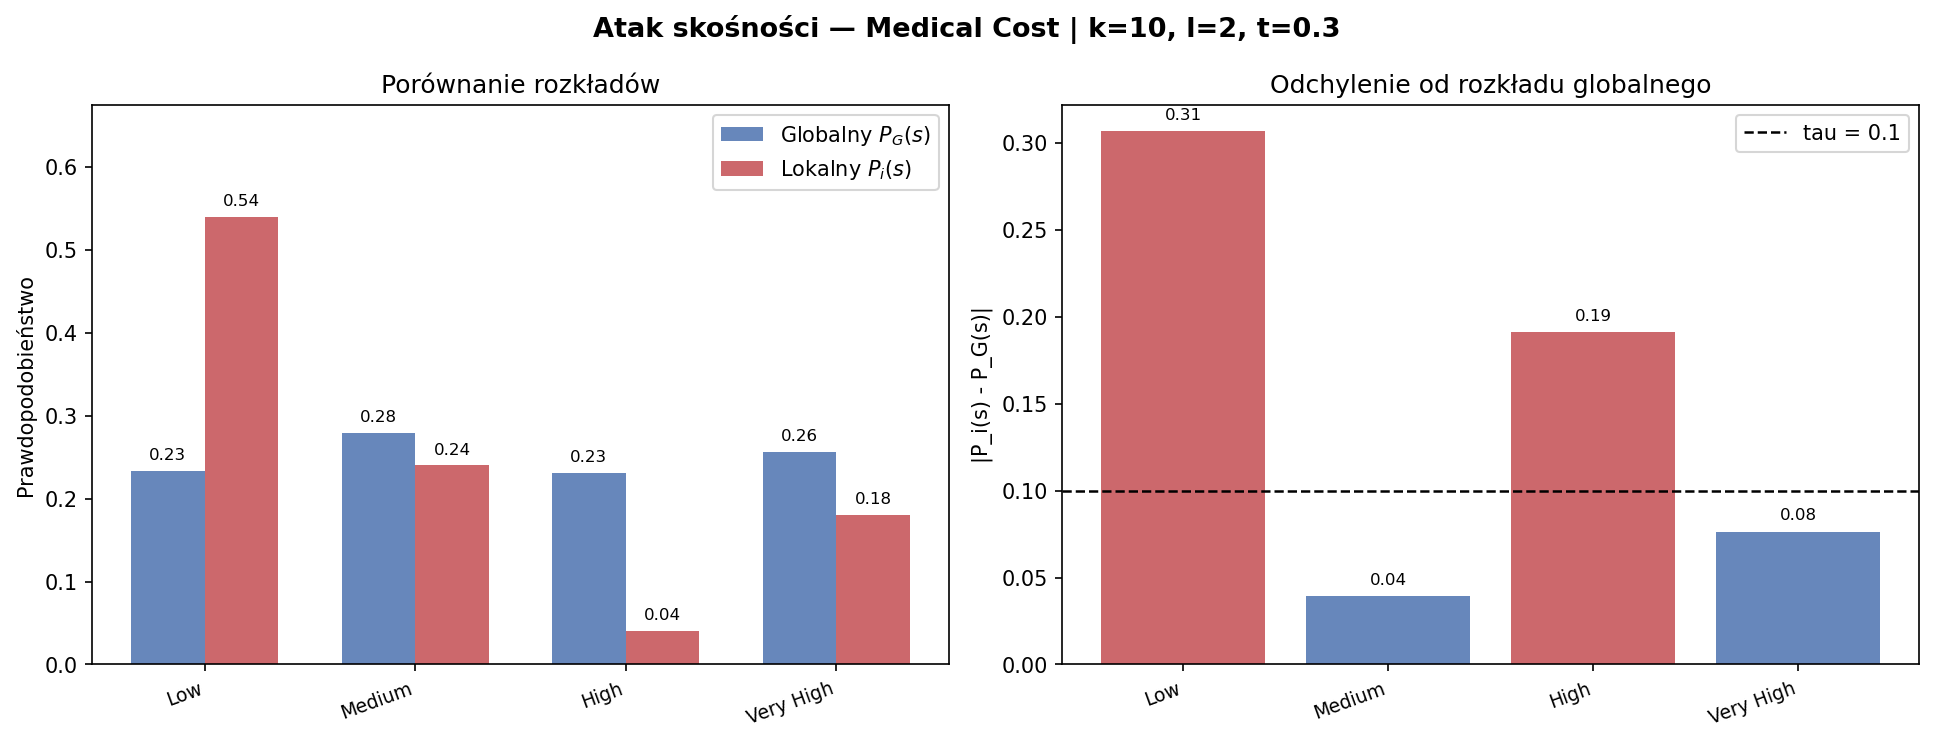
\includegraphics[width=\textwidth]{../plots/attack_medical_cost_k10_l2_t0.3.png}
    \caption{Medical Cost po t-bliskości ($t=0{,}3$). Liczba klas spada z 32 do 19
             (zachowano 62\% rekordów), ale wszystkie 19 pozostałych nadal podatne.
             Atak zmienia charakter --- teraz \texttt{Low} dominuje w podatnych klasach.}
\end{figure}

\subsection{Wykresy ataku po każdym etapie --- German Credit}

\begin{figure}[H]
    \centering
    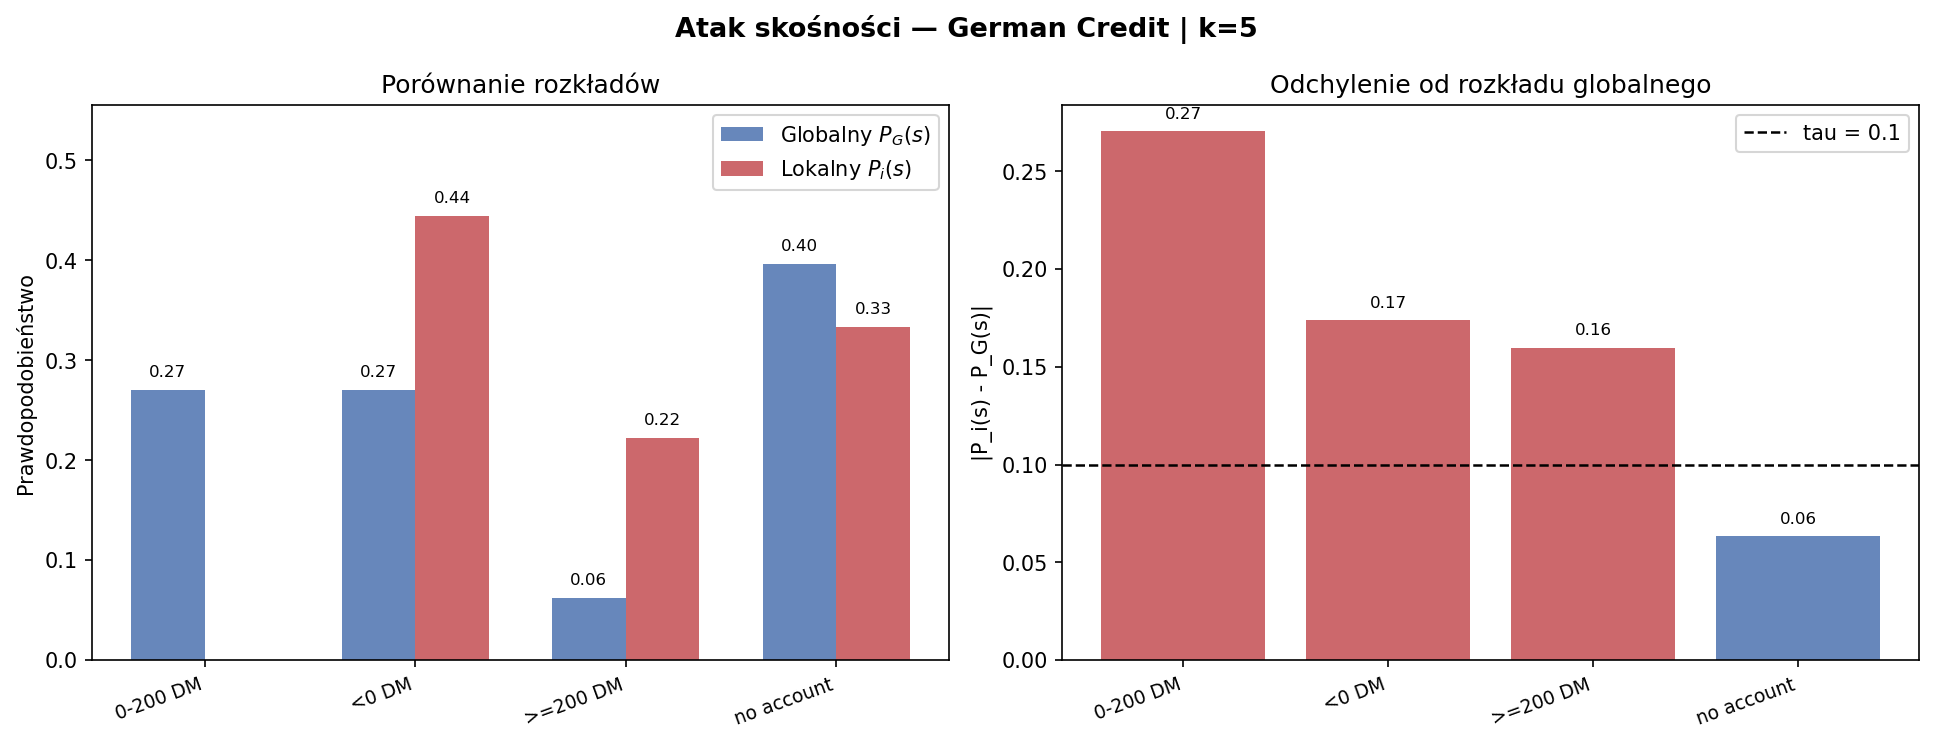
\includegraphics[width=\textwidth]{../plots/attack_german_credit_k5.png}
    \caption{German Credit po k-anonimowości ($k=5$). 13 z 20 klas podatnych (65\%).
             Podatna klasa: (male single, own, no, starszy wiek) ---
             \texttt{<0 DM}=0{,}44 vs 0{,}27 globalnie.}
\end{figure}

\begin{figure}[H]
    \centering
    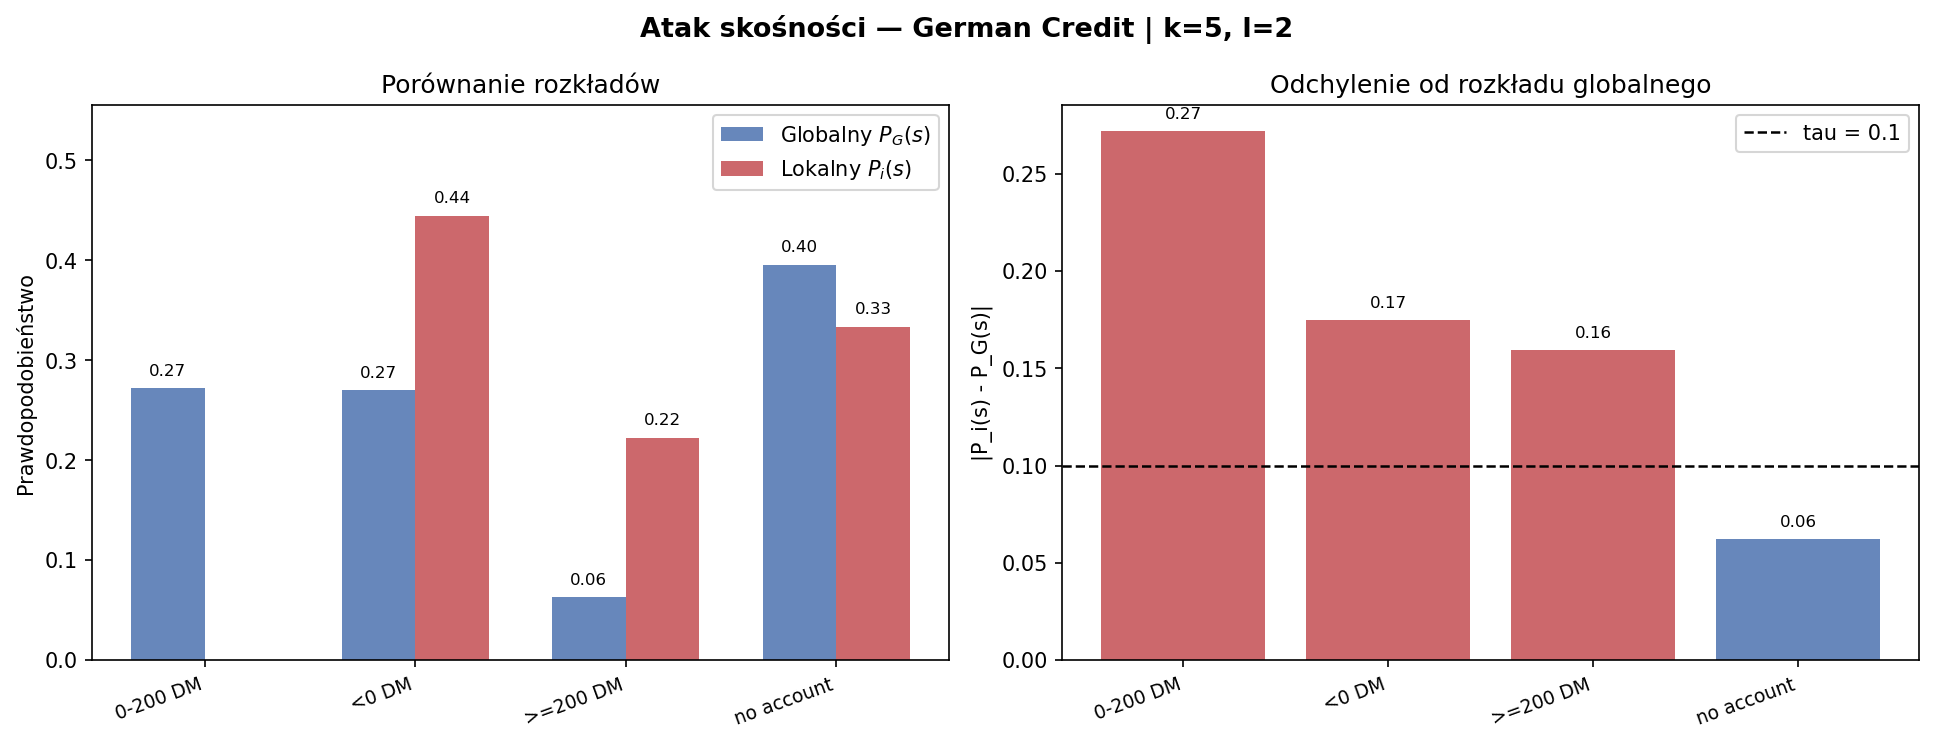
\includegraphics[width=\textwidth]{../plots/attack_german_credit_k5_l2.png}
    \caption{German Credit po l-różnorodności ($l=2$). 12 z 19 klas podatnych (63\%).
             Minimalny efekt --- l-różnorodność usuwa tylko klasy z jedną dominującą
             wartością checking\_status.}
\end{figure}

\begin{figure}[H]
    \centering
    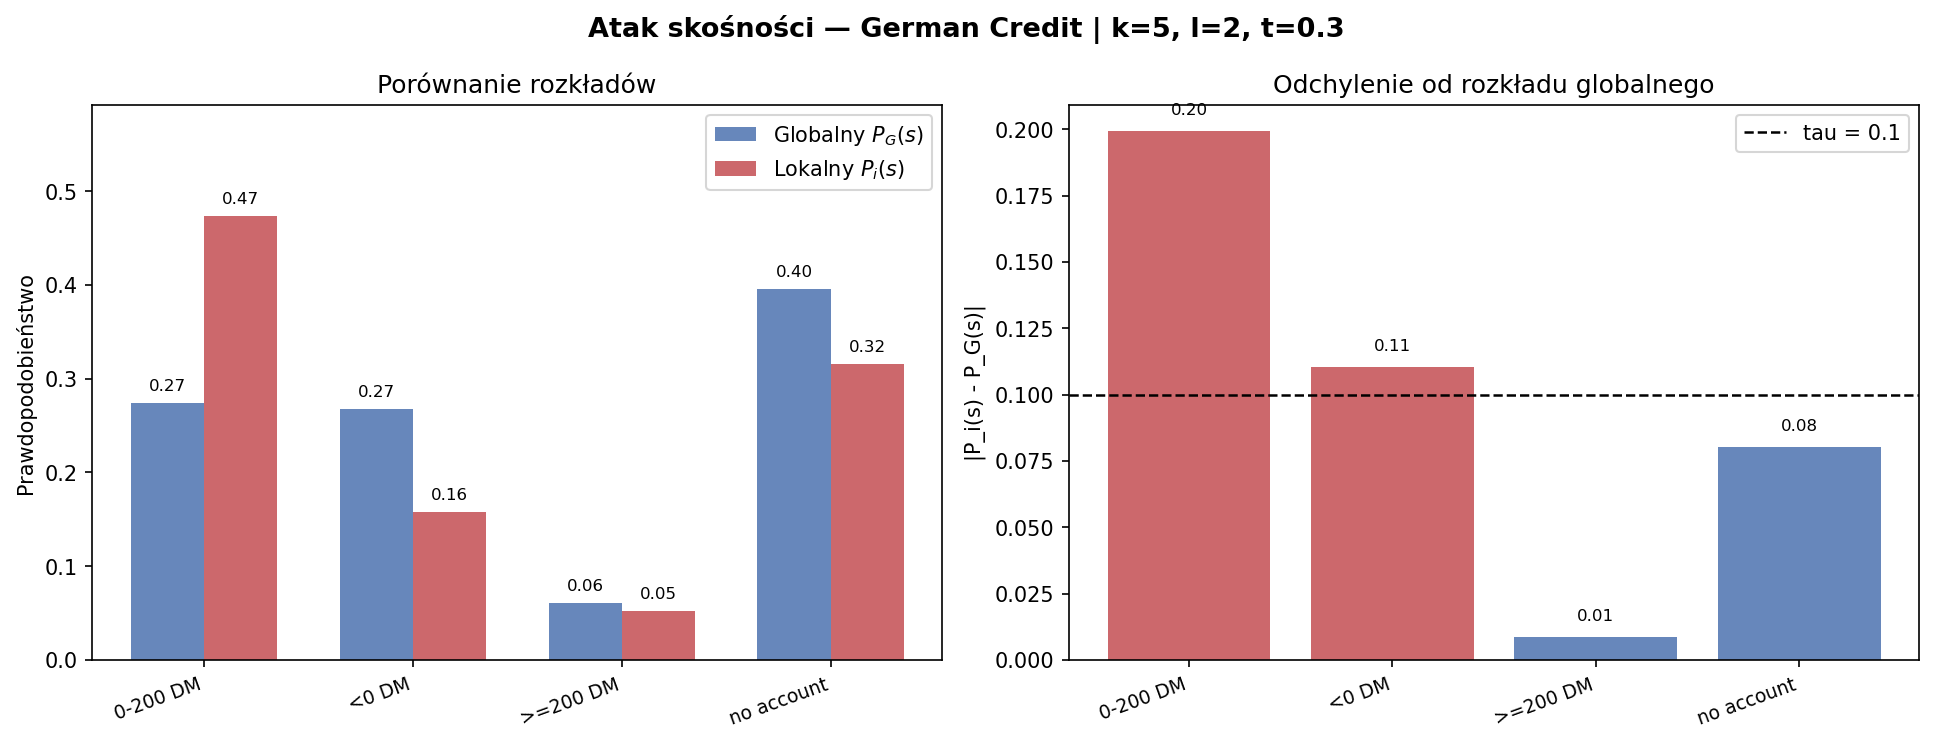
\includegraphics[width=\textwidth]{../plots/attack_german_credit_k5_l2_t0.3.png}
    \caption{German Credit po t-bliskości ($t=0{,}3$). Max odchylenie spada do 0{,}199,
             ale nadal $>\tau=0{,}10$. Do wyeliminowania ataku potrzebne
             $t \leq 0{,}10$ (zachowanie 36\% rekordów).}
\end{figure}

% =============================================================================
\section{Próg t eliminujący atak}
% =============================================================================

\subsection{Metodologia}

Dla każdego datasetu przeskanowano siatkę
$t \in \{0{,}05;\; 0{,}08;\; 0{,}10;\; 0{,}12;\; 0{,}15;\; 0{,}18;\;
0{,}20;\; 0{,}25;\; 0{,}30;\; 0{,}35;\; 0{,}40\}$.
Dla każdego $t$ zastosowano pipeline $k \to l \to t$ i sprawdzono
czy atak jest skuteczny (czy istnieje klasa z odchyleniem $> \tau$).

\subsection{Wyniki}

\begin{table}[H]
\centering
\caption{Próg $t^*$ eliminujący atak skośności ($\tau=0{,}10$)}
\begin{tabular}{lccccc}
\toprule
\textbf{Dataset} & \textbf{k} & \textbf{l} & \textbf{$t^*$} & \textbf{Rekordy przy $t^*$} & \textbf{Uwagi} \\
\midrule
Adult         & 5  & 2 & 0{,}10 & 27{,}7\% & Wąskie okno $t \in [0{,}05;\; 0{,}10]$ \\
Medical Cost  & 10 & 2 & 0{,}25 & 11{,}7\% & Przy $t<0{,}25$ brak rekordów \\
German Credit & 5  & 2 & 0{,}10 & 36{,}3\% & Najlepszy kompromis \\
\bottomrule
\end{tabular}
\end{table}

\begin{figure}[H]
    \centering
    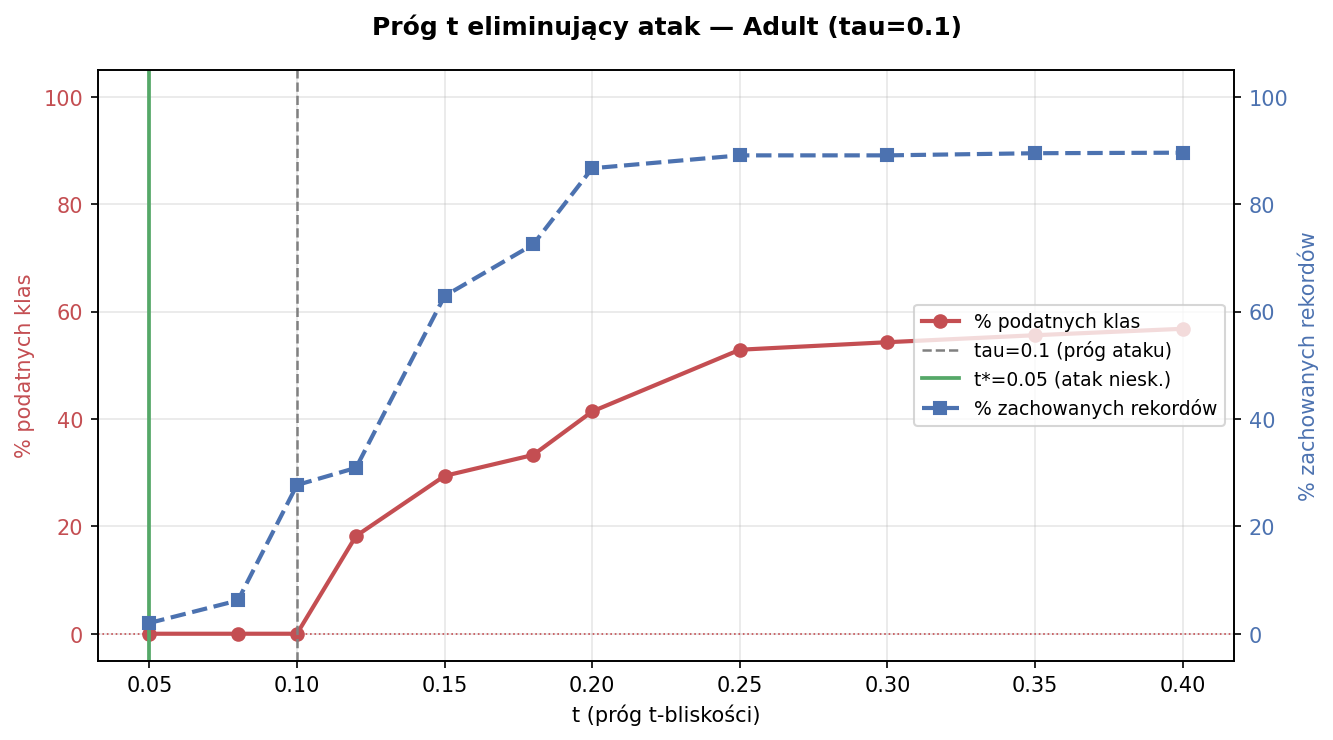
\includegraphics[width=\textwidth]{../plots/t_threshold_adult.png}
    \caption{Adult: próg $t^*=0{,}10$ eliminuje atak przy zachowaniu 27{,}7\% rekordów.
             Widoczne wąskie bezpieczne okno $t \in [0{,}05;\; 0{,}10]$ ---
             powyżej $t=0{,}12$ podatność gwałtownie rośnie.}
\end{figure}

\begin{figure}[H]
    \centering
    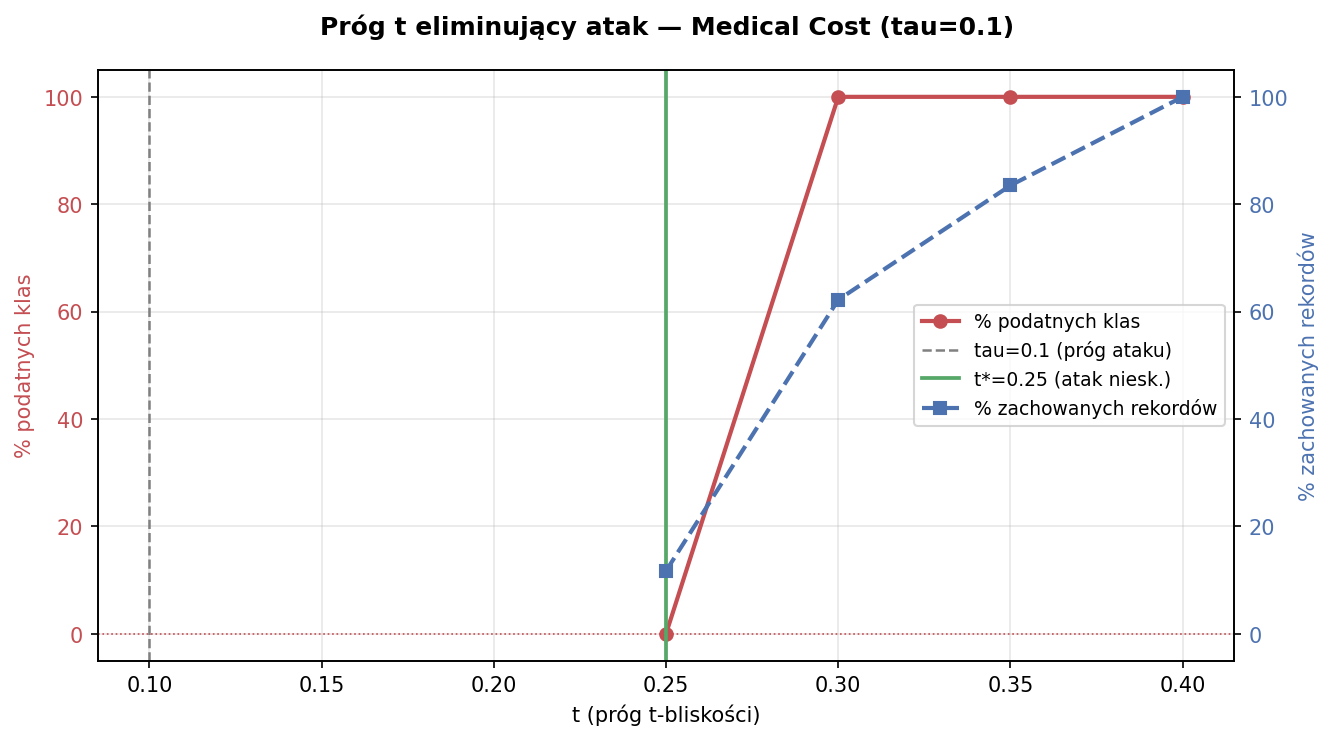
\includegraphics[width=\textwidth]{../plots/t_threshold_medical_cost.png}
    \caption{Medical Cost: $t^*=0{,}25$ z zachowaniem jedynie 11{,}7\% rekordów.
             Przy $t < 0{,}25$ t-bliskość usuwa wszystkie rekordy.
             Skokowy charakter krzywej --- brak płynnego tradeoffu.}
\end{figure}

\begin{figure}[H]
    \centering
    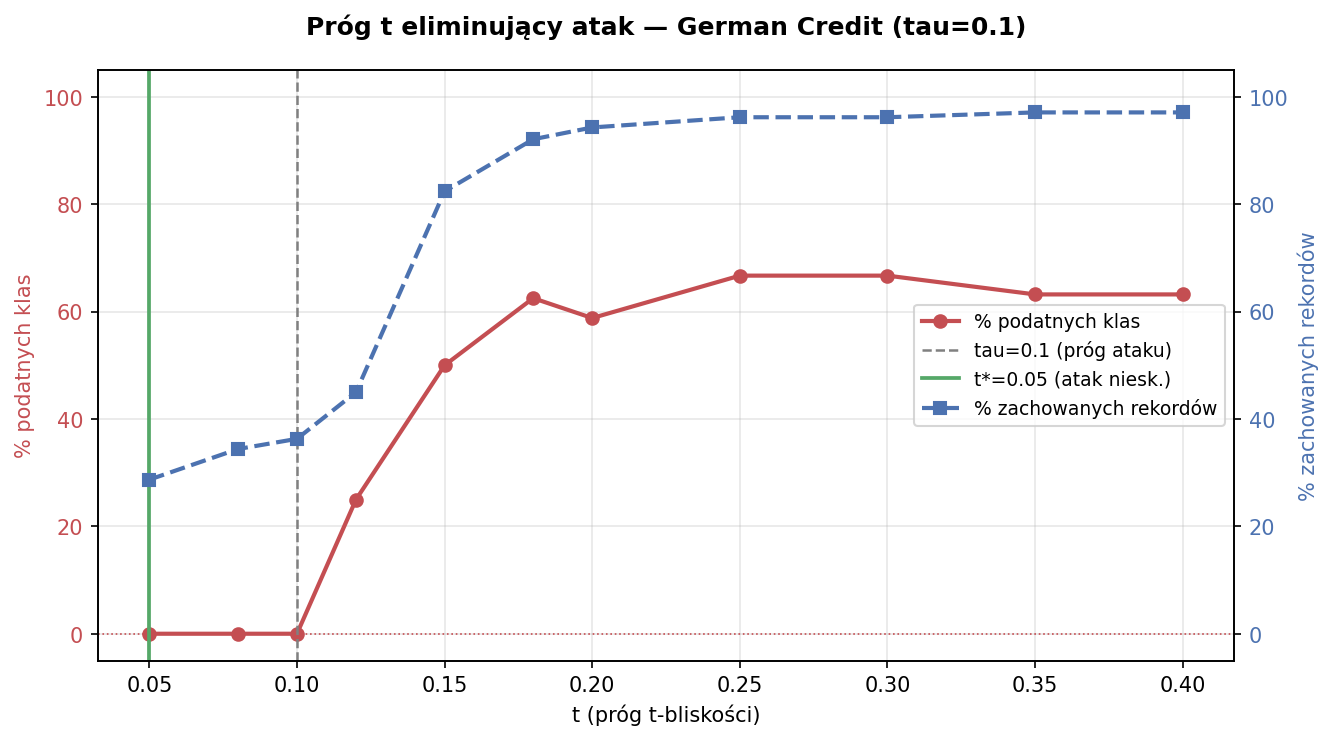
\includegraphics[width=\textwidth]{../plots/t_threshold_german_credit.png}
    \caption{German Credit: $t^*=0{,}10$ z zachowaniem 36{,}3\% rekordów ---
             najlepszy kompromis. Przy $t=0{,}10$ krzywa podatności
             dotyka zera przy 36\% użyteczności.}
\end{figure}

% =============================================================================
\section{Wnioski ogólne}
% =============================================================================

\subsection{Hierarchia ochrony}

Trzy metody tworzą hierarchię rosnącej ochrony i rosnącego kosztu:

\begin{enumerate}
    \item \textbf{k-anonimowość}: chroni przed identyfikacją konkretnej osoby,
          ale nie przed wnioskowaniem o atrybucie wrażliwym. Mała utrata danych.
    \item \textbf{l-różnorodność}: wymaga zróżnicowania atrybutu wrażliwego
          w klasie. Skuteczna gdy atrybut globalnie nierównomierny.
          Przy równomiernym atrybucie (Medical Cost) praktycznie nie działa.
    \item \textbf{t-bliskość}: bezpośrednio ogranicza odchylenie rozkładu
          lokalnego od globalnego. Gdy $t \leq \tau$, istnieje
          \emph{formalna gwarancja} że atak skośności jest niemożliwy ---
          żadna klasa nie może mieć odchylenia większego niż $t \leq \tau$.
          Empirycznie próg $t^*$ eliminujący atak może być większy niż $\tau$
          (np. Medical Cost: $t^*=0{,}25 > \tau=0{,}10$), gdy po supresji
          przypadkowo pozostają tylko klasy o małych odchyleniach.
          W obu przypadkach ochrona wiąże się ze znaczną utratą danych.
\end{enumerate}

\subsection{Porównanie datasetów}

\begin{itemize}
    \item \textbf{Adult}: duży dataset, tani k i l, ale t-bliskość $\leq 0{,}10$
          usuwa $\sim$72\% rekordów. Podatność wynika z silnej korelacji
          wykształcenia, płci i rasy z dochodem.

    \item \textbf{Medical Cost}: strukturalnie najtrudniejszy. L-różnorodność
          bezużyteczna, t-bliskość bardzo kosztowna. Wynika to z tego,
          że koszty leczenia są silnie skorelowane z paleniem (cecha poza QI).

    \item \textbf{German Credit}: najlepszy kompromis. T-bliskość z $t=0{,}10$
          eliminuje atak przy zachowaniu 36\% danych --- akceptowalny koszt
          dla wielu zastosowań.
\end{itemize}

\subsection{Praktyczne rekomendacje}

\begin{itemize}
    \item Cel: anonimizacja identyfikacyjna --- wystarczy k-anonimowość ($k \geq 5$).
    \item Cel: ochrona przed wnioskowaniem statystycznym --- dodać l-różnorodność
          (skuteczna gdy atrybut nierównomierny globalnie).
    \item Cel: ochrona przed atakiem skośności --- t-bliskość z $t \leq \tau$
          daje formalną gwarancję, jednak empiryczny próg $t^*$ eliminujący atak
          bywa większy niż $\tau$ (zależy od struktury danych).
          W każdym przypadku należy liczyć się z utratą 60--90\% rekordów.
    \item Adaptacyjne dobieranie liczby kubełków generalizacji numerycznej
          pozwala zachować więcej rekordów niż stałe progi (np. dekady wiekowe).
\end{itemize}

\end{document}
